\subsubsection{Self-supervised learning: training with simulated resections only}
\label{sec:self}

% % TODO: VERIFY THAT NOTHING IS MISSING. Move to supplementary

% The following parameters were used to generate simulated resections
% (see \sectionref{sec:simulation}):
% $f = 16$,                                           % frequency
% $\omega = 4$,                                       % octaves
% $\gamma = 0.5$,                                     % persistence
% $\zeta = 3$,                                        % scaling
% $\bm{\mu} \sim \mathcal{U}(0, 1000)$,               % offset
% $\lambda \sim \mathcal{U}(1, 2)$,                   % radii ratio
% %$r_o = 3$,                                          % ball radius for resectable hemisphere mask
% %${d_m = 4}$,                                        % median filter kernel
% and ${\bm{\sigma}_{\bm{A}} \sim \mathcal{U}(0.5, 1)}$.   % std to blur the mask
% %and $r_e = 1$.                                      % ball radius erosion of ventricles mask
% % TODO: change this
% The ellipsoid volume $v$ is sampled from volumes
% of manually segmented cavities from Rater A (see \sectionref{sec:data}).

In our first experiment, we assess the relation between the complexity of the resection simulation and segmentation performance.
We train using simulated resections on the publicly available dataset
$D\pre = \{ \X_{\text{preop}_i} \}_{i = 1}^{n\pre}$, where $n\pre = 1813$ (\sectionref{sec:data}).
% \comment{
% We use 90\% of the images in $D\pre$ for the training set
% $D\st{preop,train} = \{ \X_{\text{preop}_i} \}_{i = 1}^{n\st{preop,train}}$
% and 10\% for the validation set
% $D\st{preop,val} = \{ \X_{\text{preop}_i} \}_{i = 1}^{n\st{preop,val}}$ ($n\st{preop,train} = 1632$ and $n\st{preop,val} = 181$).
% The 133 annotated postoperative images in EPISURG are used for evaluation.

% Before training, we precompute and cache a validation set
% \begin{equation}
%     D\st{Rval}
%     = \{ T\st{Aug} \circ \phi\st{R} (\X_{\text{C}_i}) \}_{i = 1}^{n\st{Cval}}
%     = \{ ( \X_{\text{R}_i}, \Y_{\text{R}_i})          \}_{i = 1}^{n\st{Cval}}
% \end{equation}
% where $\phi\st{R}$ is the resection simulation described in \sectionref{sec:simulation} and $T\st{Aug}$ represents the preprocessing and augmentation described in \sectionref{sec:preprocessing_augmentation}.
% %Hyperparameters for $\phi\st{R}$ and $T\st{Aug}$ are specified in the supplementary material\textcolor{red}{[TODO?]}.
% }
We use 90\% of the images in $D\pre$ for the training set $D\st{pre,train}$ and 10\% for the validation set.
The 133 annotated postoperative images in EPISURG are used for evaluation.

At each training iteration, $b$ images from $D\st{pre,train}$ are loaded, resected, preprocessed and augmented to obtain a mini-batch of $b$ training instances
$\{ ( \X_{\text{preop}_i}, \Y_{\text{cavity}_i}) \}_{i = 1}^{b}$.
Note that the resection simulation is performed on the fly, which ensures that the network never sees the same resection twice during training.

All models were trained for 60 epochs, using an initial learning rate of $10^{-3}$.
We select the model with the lowest mean validation loss obtained during training for evaluation.


\begin{table}[hb!]
    \centering
    \floatconts
    {tab:self}
    {\caption{%
        Quantitative evaluation of models trained with simulated resections only.
        The labeled images in EPISURG are used for evaluation.
        \ac{DSC} is expressed as `median (interquartile range)'.
    }}
    {
    \begin{tabular}{cccc}
        \toprule
        \centering \textbf{White matter lesion} &
        \centering \textbf{Blood products} &
        \centering \textbf{Cavity shape} &
        \textbf{DSC} \tabularnewline
        \midrule
                        % No &                      No &                 Noisy &                    No &  00.0 (00.0)  \\  % 24 -
                        No &                      No &                Cuboid &  57.9 (73.1)  \\  %  5 -
                        No &                      No &             Ellipsoid &  79.0 (20.0)  \\  %  9 -
                        No &                      No &                 Noisy &  \textbf{80.5 (18.7)}  \\  %  2 - 30
                        No &                     Yes &                 Noisy &  79.6 (16.5)  \\  % 21 - compare with problematic cases in 2!
                       Yes &                      No &                 Noisy &  78.2 (20.3)  \\  % 16 -
                       Yes &                     Yes &                 Noisy &  78.0 (18.0)  \\  % 18 -
        \bottomrule
    \end{tabular}
    }
\end{table}


\paragraph{Effect of resection shape}

To investigate the effect of the simulated cavity shape on model performance, we modify $\phi\simul$ to generate cuboid- (\figureref{fig:exp_shape_cuboid}) or ellipsoid-shaped (\figureref{fig:exp_shape_ellipsoid}) resections, and compare the performance with the baseline ``noisy'' ellipsoid (\figureref{fig:exp_shape_noisy}).
The cuboids and ellipsoid meshes are not perturbed using simplex noise, and cuboids are not rotated.

%he performance of the baseline model is only marginally better than the model trained with rotated ellipsoids ($p = 0.123$) (\tableref{tab:self}).
%The model trained with cuboid-shaped resection cavities performed significantly worse than the baseline model ($p < 10^{-8}$).
%Model performance is poor when the simulated cavities are cuboids, and best results were obtained using ellipsoids perturbed with procedural noise.

Best results were obtained by the baseline model, trained using ellipsoids perturbed with procedural noise, that we denote $\fp{sim}$.
Models trained with cuboids and rotated ellipsoids performed significantly ($p < 10^{-8}$) and marginally ($p = 0.123$) worse (\tableref{tab:self}).



% $ seed=21 && shape="noisy" && debug_dir="/tmp/debug_dir_${seed}_${shape}" && resect /Users/fernando/git/ijcars-2020/nii/t1.nii.gz /Users/fernando/git/ijcars-2020/nii/t1_seg_gif.nii.gz $debug_dir/resected.nii.gz $debug_dir/label.nii.gz -miv 20000 -mav 20000 -d $debug_dir -s $seed -r 25 -18 74 --shape $shape

% Slice 119
\begin{figure}
    \centering
    \floatconts
    {fig:exp_shape}
    {\caption{%
        Simulation of resection cavities with increasing shape complexity:
        cuboid (a),
        ellipsoid (b)
        and ellipsoid perturbed with simplex noise (c).
    }}
    {
        \subfigure{%
            \label{fig:exp_shape_cuboid}%
            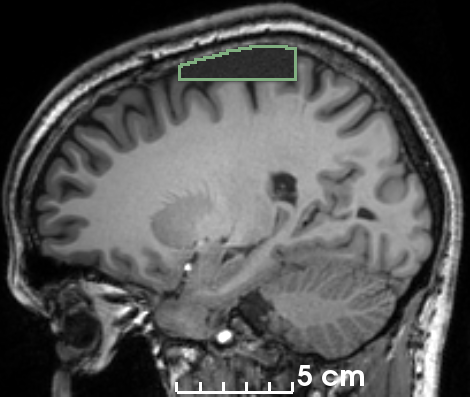
\includegraphics[width=0.3\linewidth]{exp_shape_cuboid}
        }%
        \subfigure{%
            \label{fig:exp_shape_ellipsoid}%
            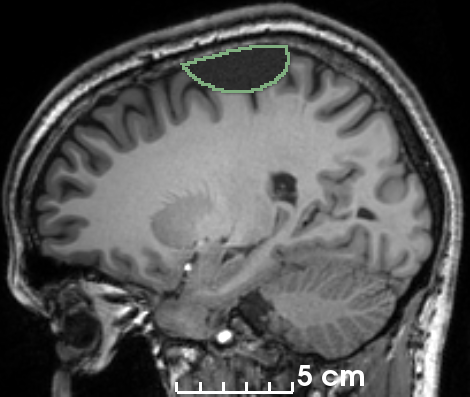
\includegraphics[width=0.3\linewidth]{exp_shape_ellipsoid}
        }%
        \subfigure{%
            \label{fig:exp_shape_noisy}%
            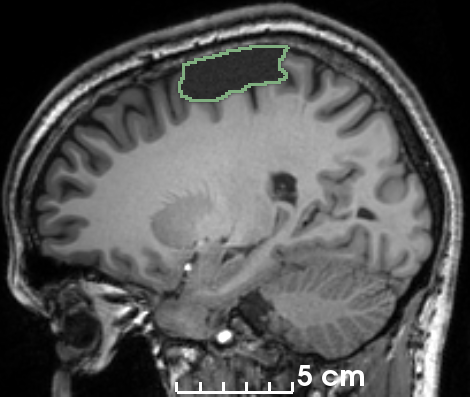
\includegraphics[width=0.3\linewidth]{exp_shape_noisy}
        }
    }
\end{figure}



\paragraph{Effect of resection texture}

We investigate the effect of simulating additional postoperative phenomena such as white matter lesions around the cavity and blood products inside the cavity (\figureref{fig:exp_texture}).

Adding either of these effects did not improve results, but the superiority of the baseline model with respect to the models trained with white matter lesions ($p = 0.163$), blood products ($p = 0.323$) or both ($p = 0.054$) was not statistically significant (\tableref{tab:self}).
This may be due in part to the relative rarity of these additional effects in the evaluation dataset.

%  $ seed=21 && shape="noisy" && debug_dir="/tmp/debug_dir_${seed}_${shape}_wm_bc" && resect /Users/fernando/git/ijcars-2020/nii/t1.nii.gz /Users/fernando/git/ijcars-2020/nii/t1_seg_gif.nii.gz $debug_dir/resected.nii.gz $debug_dir/label.nii.gz -miv 20000 -mav 20000 -d $debug_dir -s $seed -r 25 -18 74 --shape $shape -w -b

% Slice 120
\begin{figure}
    \centering
    \floatconts
    {fig:exp_texture}
    {\caption{%
        Simulation of resection cavities with increasing texture complexity:
        baseline (a),
        blood products (b),
        white matter lesion (c)
        and both (d).
    }}
    {
        \subfigure{%
            \label{fig:exp_texture_baseline}%
            \includegraphics[width=0.24\linewidth]{exp_texture_baseline}
        }%
        \subfigure{%
            \label{fig:exp_bc}%
            \includegraphics[width=0.24\linewidth]{exp_texture_bc}
        }%
        \subfigure{%
            \label{fig:exp_texture_wm}%
            \includegraphics[width=0.24\linewidth]{exp_texture_wm}
        }%
        \subfigure{%
            \label{fig:exp_shape_wm_bc}%
            \includegraphics[width=0.24\linewidth]{exp_texture_wm_bc}
        }%
    }
\end{figure}